\chapter{Background Research}
\label{CHAP_SECOND}
\centerline{\rule{149mm}{.02in}}
\vspace{2cm}
This chapter is intended to give an overview of the current research landscape, and to summarise the core technologies and concepts which form a basis for this project. The chapter will discuss trends toward Cloud Computing, how it is relevant to Data Processing, and key technologies which have been developed in this area, giving a foundation for further investigation into the efficiency of Data Processing techniques and how they are impacted by the Cloud. 

\section{Cloud Computing}
Cloud Computing is the latest major infrastructure paradigm which looks to deliver on the promise of Utility Computing. In practice, the term `Cloud Computing' is ambiguous. Whilst no clear definition exists many experts agree that the cloud exhibits the core benefits of Utility Computing such as elasticity and scalability, whilst making heavy use of virtualisation and pay-per-usage business models \cite{vaquero2008}.

Elasticity in clouds refers to the ability for a user to dynamically select the amount of computing resources they require, allowing them to scale their applications according to demand. The resources that can be acquired are essentially limitless from the user's perspective \cite{mell2011nist}. 

Elasticity represents a dramatic shift from the `traditional' method of building and deploying applications. Rather than purchasing and provisioning hardware and acquiring physical space (such as a data centre), a user can use a Cloud Service Provider. This allows for greater flexibility in business and application development, as users can cope with unpredictable or inconsistent levels of demand. An example of where this flexibility would benefit a company is in the case of an online store. A store may receive fluctuating traffic throughout a year, such as being particularly busy around the Christmas period. It would be economically inefficient for the store to purchase extra servers to cope with demand over the festive period, as they would be redundant for the majority of the year, but they must improve hardware capability in order to take advantage of the extra business. The inherent flexibility from the elasticity of the cloud would allow the store to simply acquire new computing capacity from their Cloud Service Provider on a temporary basis, giving them the capability of accommodating with the peak traffic but not using (or paying for) the extra resources when they are not needed. Having this scalability is seen as a core benefit of Cloud Computing.

A Cloud Service Provider is an organisation that provides access to Cloud Computing resources. They manage the underlying hardware, and typically provide APIs and other methods for a user to manage their resources. Some of the largest Cloud Service Providers are Amazon through AWS (Amazon Web Services), Microsoft through Windows Azure and Google through Google Apps.

A Cloud Service Provider does not have to be an external organisation, but when they are they typically use pay-per-usage business models. Rather than pay a fixed monthly cost, or have a one-off license fee, customers will pay the Cloud Service Provider for the resources they use (usually on a per-hour basis). For example, a `Medium' size Virtual Machine costs £0.077 an hour from Windows Azure \cite{AzurePricing}. This allows businesses to only pay for the resources that they need.

\subsection{Related Ideas}
\subsubsection{Utility Computing}
Utility Computing is the idea that households and businesses could outsource their demand to external companies, who provide the relevant amount of service on a pay-per-usage basis. Customers would access computing resources over a network, and would pay for the length of computing time that they use.

This is analogous to other utilities such as Gas or Electricity. In the case of Electricity, power is provided from the National Grid and the customer pays for how much they use. This allows a customer change the amount of power they require without having to pay a fixed cost (for example, using less electricity when they are on holiday).

Utility Computing is an established concept, with leading thinkers such as Leonard Klienrock (part of the original ARPANET project) referencing it as early as 1969 \cite{319}. Various technologies have emerged which offer some attributes associated with utility computing, with Grids and Clouds appearing to be the most promising \cite{buyya2008market}.

\subsubsection{Virtualisation}
Virtualisation is one of the key enabling technologies behind Cloud Computing. It abstracts away the details of the physical hardware and allows Cloud Service Operators to run several virtual machines on one physical machine \cite{zhang2010cloud}, completely independently of one another. This allows for customers applications and the physical hardware to be consolidated, utilising resources more efficiently and making it financially feasible to run a cloud \cite{foster2008cloud}. 

The configurability afforded by virtualisation is another property essential to Cloud Computing. It allows Cloud Service Providers to support a diverse range of applications, which may have different requirements (high compute, high memory, etc). Virtualisation allows this to be achieved, as it would be prohibitively costly at hardware level \cite{foster2008cloud}. 

The reliability of a cloud can also be improved through the use of virtualisation techniques. Virtual Machines can be backed up, migrated and replicated simply, allowing applications to recover from hardware failure. 

\section{Cloud Computing Service Models}
Depending on the scenario, the Cloud offers several different service models. These models allow for clients to provision services in a different manner depending their requirements.

The different service models provide different levels of abstraction for the user. In Infrastructure as a Service, the user has full control over the machines that they acquire from the Cloud Service Provider, where in Software as a Service they are given less control, and need not worry about the underlying hardware whatsoever.

\subsection{Infrastructure as a Service}
Infrastructure as a Service (IaaS) provides an abstraction on top of a virtualisation platform, so that the client does not need to worry about what method of virtualisation is being used, and does not have to learn about the underlying technologies \cite{amies2012}.

Clients can request Virtual Machines in varying configurations, and a Virtual Infrastructure Manager will provision an appropriate Virtual Machine on a physical machine which has capacity. In addition to allowing users to provision virtual machines, IaaS systems may allow a user to configure other infrastructure elements, such as virtual networks. 

This provides a great deal of control to the user, as they are essentially renting a machine of a requested specification for a short period of time. They are free to install whatever Operating System and software on the machine as required, and can configure it in essentially any way. 

An example of an Infrastructure as a Service provider would be Amazon EC2 \cite{amazonEC2}. Amazon provide a variety of different Virtual Machine types, including those specialising in High Performance Computing or applications requiring a large amount of memory. Virtual Machines can use a range of images provided by Amazon (including Windows and various distributions of Linux), or users can create and upload their own custom Virtual Machine images. 

\subsection{Platform as a Service}
Platform as a Service (PaaS) is a higher level abstraction which allows applications to be built and deployed without worrying about the underlying Operating System or runtime environment \cite{intelPaaS}. The user still specifies the resources required, but no longer has to manually manage the virtual machines. The Cloud Service Provider will maintain the machines, providing the necessary software (Operating Systems, Web Servers, etc) and updating them frequently.

The advantage of PaaS is that it allows users to deploy their own applications, without having to worry about maintaining the underlying infrastructure. Whilst this decreases the control the user has over the deployment environment, it reduces the complexity of managing the infrastructure themselves. 

PaaS offerings may also provide supplementary services to users, such as health and availability monitoring, or auto-scaling.

Windows Azure is an example of a Platform as a Service provider \cite{azure}. Whilst they provide Infrastructure as a Service offerings, they also provide Platform as a Service capabilities through Windows Azure Web Sites. Windows Azure Web Sites allow users to upload applications written in a variety of web technologies (ASP.NET, Python, PHP, Node.js) and have them hosted in the Windows Azure runtime environment. This means the client does not manually have to manage web servers, frameworks and other necessary technologies.

\subsection{Software as a Service}
Software as a Service (SaaS) refers to providing access to applications over the internet on-demand \cite{zhang2010cloud}. Software is centrally hosted by the Cloud Service Provider, and clients can access the application through a web browser or other form of client. As the software is centrally hosted, Cloud Service Providers can handle updating the software for all users, ensuring all users benefit from bug fixes or additional features. 

Software as a Service applications can reduce the cost of deploying and using software for an organisation as they don't have to purchase their own hardware, install and configure software, and can avoid having technical support staff. An example of a successful Software as a Service application is Salesforce \cite{salesforce}. Salesforce is a Customer Relationship Management tool which charges organisations per user, making it a viable choice for small businesses. Salesforce can be accessed through a web browser, enabling customers to use their software regardless of location or device. 

\section{Cloud Computing Deployment Models}
Cloud Services can be deployed in several different ways. The National Institute of Science and Technology defines 4 Cloud Computing deployment models \cite{mell2011nist}.

\subsection{Public Cloud}
A public cloud is designed to for use by the general public. A public cloud will typically be owned by a third-party Cloud Service Provider such as Microsoft or Amazon, and will serve lots of different individuals and organisations. 

The benefit of a public cloud is that physical infrastructure is completely managed and maintained by the Cloud Service Provider, reducing the effort required to provision computing resources and therefore maximising the benefit of the cloud.

\subsection{Private Cloud}
A private cloud is designed for use by one organisation. This allows individual components of an organisation (such as departments, product groups or engineering teams) to utilise the benefits of Cloud Computing, whilst allowing the organisation to maintain control over the computing resources. A private cloud allows an organisation to completely tailor the cloud to their unique requirements, including specialised hardware, specific Platform/Software as a Service offerings and control over the permissions clients of the cloud environment have.

A private cloud can also be necessary in overcoming concerns about security and data governance. One of the major disadvantages of a public cloud is a lack of control over data (real or perceived). It may not be possible to ascertain where data is geographically located (and therefore what legislation applies to it), and companies may simply not trust confidential information with a third-party Cloud Service Provider.

Whilst a private cloud still requires an organisation to acquire, provision and manage hardware (rather than outsourcing to a third-party Cloud Service Provider), it can still provide a reduction in cost over time. A private cloud allows centralisation of an organisations computing resources, allowing components of the organisation to use resources elastically as required from the central private cloud, rather than duplicating necessary computing infrastructure.

\subsection{Community Cloud}
A community cloud is developed by several organisations that have shared requirements. It allows them to pool together computing resources to the benefit of all organisations involved, reducing the investment needed for a private cloud. Organisations may opt to develop a community cloud to reduce dependency on a public cloud provider, mitigating the privacy and security concerns often cited as being a problem for public clouds, and allowing the resulting cloud system to be tailored to take in to account legislative or administrative restrictions which might be part of some industries or other organisational groups.

Whilst creating a community cloud provides tangible security and customisability benefits over a public cloud, and cost benefits over developing a private cloud system, they also have their issues. Community clouds can make it more difficult to deal with standard distributing computing issues such as latency and resource management, and additional security requirements may be needed \cite{briscoe2009digital}. 

\subsection{Hybrid Cloud}
A hybrid cloud is a composition of 2 other cloud types (public, private and community). Typically, a hybrid cloud uses technology to enable data and applications to be transported between clouds. An example of a hybrid cloud solution would be a private cloud, which utilises a public cloud if it runs out of resources. This allows the private cloud to exhibit the same elasticity benefits of a public cloud, appearing to clients as though it has essentially limitless resources (whilst actually just making use of a public cloud for overflow capacity).

It may be difficult to create a hybrid cloud in some situations as the technologies used may be complete distinct and difficult to combine. There may also be concerns about data security and privacy. Business rules may have to be defined which specify (for example) what types of data can be stored on a public cloud, and what types of data are too sensitive and must remain private at all costs. 

\section{Big Data}
The term `Big Data' refers to large scale data sets which present new problems for the processing and analysis of data. These datasets are often too large to be comfortably worked with using standard tools for statistical analysis \cite{snijders2012big}. Sources of Big Data are diverse; datasets can be from science, industry, social networking sites or various other sources. Consider the following:

\begin{itemize}
	\item In 2011, Facebook had 30 PetaBytes of data used for performing analytics \cite{facebookBigData}.
	\item The Large Hadron Collider generates ~25 PetaBytes of data annually \cite{lhcData}.
	\item Phase one of the 1000 Genome Project has a dataset of 180 TeraBytes of human genetic information \cite{genomeData}.
	\item In 2008, Google were capable of processing 20 PetaBytes of data a day \cite{dean2008mapreduce}.
\end{itemize}

\subsection{Challenges}
Big Data introduces several challenges which make the use of traditional analysis tools and techniques infeasible.

\subsubsection{Scale}
The defining characteristic of Big Data problems is their massive scale. Typical problems may require processing datasets in the magnitude of PetaBytes of information. This makes it unrealistic to process the data in serial, as it would take far too long. Data processing techniques designed for Big Data problems must process information in parallel. 

The scale of the data also makes storing data on a single machine unrealistic. Whilst the capacity of hard drives has been increasing over time, the speed of I/O has not increased by the same factor \cite{white2009hadoop}. This makes it time consuming to read an entire dataset off of one physical disk, even if a disk exists with enough capacity. 

Unfortunately, the alternative approach of distributing data across multiple machines also has issues. Using a higher number of nodes increases the likelihood that one of those nodes will fail, which could lead to irrecoverable data loss. In order to prevent this, systems for processing Big Data should be designed to be fault tolerant, usually by introducing redundancy.

\subsubsection{Predictability}
Not all Big Data is static. There has been increasing interest in performing sentiment analysis on social networks to predict the results of real-world events such as box office revenues \cite{asur2010predicting}, financial markets \cite{bollen2011twitter}, or surveys on political opinion \cite{o2010tweets}. 

It can be difficult to predict the quantity of data which may need to be processed when analysing real-time data, such as that gathered by Twitter. In August 2013 Twitter experienced an unexpected increase in traffic, leading to a new record for the number of tweets in a second \cite{tweetRecord}. This highlights the potentially unpredictable nature of real-time data analytics. 

The challenges of predicting resources required for real time data analytics show the advantage of using Cloud Computing for data processing. The elastic nature of clouds would allow resources to be dynamically acquired when an unpredictable increase in data occurs. 

\subsubsection{Data Heterogeneity}
It is very rare for different data sources represent data in the same way. Where data is processed from multiple sources, the lack of standard methods of storing data can make it difficult to develop accurate processing techniques \cite{cuzzocrea2011analytics}. 

A lack of structure in data can also cause problems with analysis. Much of the data used in large scale processing is strongly unstructured (social network data, text from articles, etc) which can cause issues with processing techniques. For example a simple data processing task which counts the frequency of words in a text document may produce inaccurate results if there are spelling mistakes in the corpus. 

\section{MapReduce}
MapReduce is a programming paradigm designed as a generalised solution to processing large scale datasets \cite{dean2004mapreduce}. A programmer specifies both a \textit{map} and \textit{reduce} function, a set of input data, and a location for the output. A MapReduce runtime  determines how to distribute the task, taking the data and dispersing it amongst its nodes, enabling the data to be processed in parallel.

The key advantage of MapReduce is that it provides an abstraction on top of concurrent programming. This allows a developer to specify what they want to do to the data (in terms of the \textit{map} and \textit{reduce} functions) without having the obscuring the code and having the cognitive overhead of handling common concurrency issues, such as fault tolerance, data distribution, and safe parallelism without the risk of problems such as race conditions and deadlocks. 

The MapReduce method of performing distributed parallel data processing is inspired by the \textit{map} and \textit{reduce} functions present in many functional programming languages \cite{dean2004mapreduce}. 

\subsection{Map}
The first function that a developer provides is the \textit{map} function.

$$ map = (k, v) \rightarrow list(k^{\prime}, v^{\prime}) $$

The \textit{map} function receives a key and a value as input (an \textit{Input Pair}), and returns a list of (different) keys and values (a list of \textit{Output Pairs}. The MapReduce runtime will take all output pairs with the same key, and combine them in to a list before passing the resulting values to the \textit{reduce} function. The reduce function therefore receives an argument of type $ (k, list(v)) $.

\subsection{Reduce}
The \textit{reduce} function is the second function provided by the developer. 

$$ reduce = (k, list(v)) \rightarrow list(v^{\prime}) $$

A \textit{reduce} function merges values together to produce a smaller list of values. Typically, the reduce function is an aggregate function, returning either 1 or 0 results (such as sum, average, etc). 

\subsection{Word Counting Example}
A common MapReduce operation is word counting. The following pseudo-code implementation of the \textit{map} and \textit{reduce} functions for counting words in a document obtained from \cite{dean2004mapreduce}.

\begin{algorithm}
\caption{Map function for word counting}
	\begin{algorithmic}
		\REQUIRE key: document name
		\REQUIRE value: document contents

		\FORALL{w in value}
			\STATE EmitIntermediate(w, 1)
		\ENDFOR
	\end{algorithmic}
\end{algorithm}

The \textit{map} function takes a document, and returns a number of Key/Value pairs, where the key is a word appearing in the document, and the value is 1. The runtime environment will then cluster the values together where the keys match. Each word will therefore have a list of 1's, with the length of the list indicating how many times the word has occurred.

\begin{algorithm}[H]
\caption{Reduce function for word counting}
	\begin{algorithmic}
		\REQUIRE key: a word
		\REQUIRE value: a list of counts
		\STATE result = 0
		\FORALL {v in values}
			\STATE result += v
		\ENDFOR
		\RETURN result
	\end{algorithmic}
\end{algorithm}

The reduce function takes the list of values (all of which are 1) and sums them together. This gives a total number of times the word has occurred in the document.

\subsection{Disadvantages}
The primary criticism of MapReduce is that it provides a limited programming framework \cite{zaharia2010spark}. Whilst the MapReduce paradigm is a relatively general concept which applies to many types of application, not all problems can be formulated in a way which is compatible with MapReduce. The MapReduce process consists of a static \textit{map} operation, performed across the data, and a static \textit{reduce} operation performed subsequently. The \textit{map} and \textit{reduce} functions are both stateless. 

This imposes limitations on the types of problem which can be solved by MapReduce. If it is not possible to formulate a \textit{map} and \textit{reduce} function for a problem, it cannot be solved by the MapReduce paradigm. Alternatively, whilst it may be possible to express a data processing task in terms of \textit{map} and \textit{reduce}, it does not always provide the most fluent or efficient method of solving the problem. 

Prominent examples of this type of algorithm can be found in Machine Learning, where problems are often iterative in nature. Iterative tasks, such as K-Means Clustering can be implemented using the MapReduce paradigm \cite{zhao2009parallel}, but often require multiple passes of the \textit{map} and \textit{reduce} functions, which causes a significant performance penalty as data must be loaded from the disk every iteration.

\subsection{Hadoop}
Hadoop is an Open Source implementation of the MapReduce programming paradigm \cite{hadoop}. It consists of several modules designed to overcome the problems associated with large scale data processing. In addition to the MapReduce programming model (Hadoop MapReduce), the Hadoop platform also has a distributed file system (HDFS) and a resource management and scheduling component (Hadoop YARN). 

Hadoop is a particularly popular implementation of the MapReduce interface in the data processing community, emerging as the de-facto standard implementation of MapReduce \cite{qin2013reflection}.

\section{PACTs}
\textbf{Pa}rallelization \textbf{C}ontrac\textbf{t}s (PACTs) is an alternative programming paradigm which is a generalization of the MapReduce concept \cite{battre2010socc}. The aim of PACT is to overcome the perceived weaknesses in the MapReduce paradigm, whilst still providing a generic enough framework to represent any data processing task. PACT sets out to improve MapReduce by observing that the \textit{map} and \textit{reduce} functions alone cannot represent all data processing tasks in a natural or efficient way, that MapReduce does not provide flexibility in the order of operations (strictly a \textit{map} followed by a \textit{reduce}) and that MapReduce makes no assumption about the user defined functions, limiting the scope of potential optimizations.

PACT aims to solve these issues in 2 ways. It introduces the concept of Parallelization Contracts, which define properties of a user defined functions input and output data, and it represents the data flow of a data processing job as a Directed Acyclic Graph (DAG), rather than strictly as a \textit{map} and \textit{reduce} task.

\subsection{Processing Tasks}
A data processing job can be described as a set of tasks, where each task performs a transformation on the data. A processing task has 3 core components.

A data processing task acts upon a list of records. Unlike the classic MapReduce paradigm, input is not restricted to Key/Value pairs. A record can consist of any number of fields, each which can be either a key or value. All fields must be capable of being serialized and deserialized, and fields defined as keys must be capable of being compared with other keys. 

\subsubsection{Input Contract} 
A task can be described as consisting of multiple Parallelization Units (PUs). A PU is a core block of computation which must be performed in serial. PUs are isolated from one another, and do not require communication, meaning that they can be distributed across different nodes and can be ran in parallel to one another. PACT specifies a set of Input Contracts which define how a problem is broken down into PUs. The Input Contract is therefore key in determining how the problem is made parallel and distributed between nodes.

The PACT Programming Model provides 5 Input Contracts \cite{alexandrov2010massively}.

\begin{itemize}
    \item \textbf{Map} takes a list of records and creates a PU for each individual record. This allows every record to be processed in parallel. The Map Input Contract is typically used for transforming or filtering data.
    \item \textbf{Reduce} takes a list of records and groups them by record key. It then creates a PU for each group, allowing the resulting subsets to be processed in parallel. The Reduce Input Contract is often used for aggregating data, performing functions like sum or average.
    \item \textbf{Cross} is a multi-input contract, taking 2 lists of records. It takes the Cartesian product of the 2 lists, and creates a PU for each element in the resulting set. This allows every combination of input to be processed in parallel.
    \item \textbf{CoGroup} takes 2 lists of records and groups them by key. A PU is then generated for every resulting group. This is similar to the Reduce Input Contract, but it operates across 2 lists rather than 1.
    \item \textbf{Match/Join} takes 2 lists and matches records from the first with records from the second based on whether they have the same key. A PU is generated for every resulting pair of records. This is conceptually similar to an equi-join operation.
\end{itemize}

\subsubsection{User Defined Function}
The User Function is the programmer defined function which will be executed on the data. This may be counting the frequency of words, searching for a particular string, or various other things. The arguments that the User Function will receive are based on the input contract - if a Map Input Contract is used, the User Function will receive an individual record. If a Reduce Contract is used, the User Function will receive a group of records with similar keys.

\subsubsection{Output Contracts}
An Output Contract is an optional component of a data processing task. An Output Contract is used to provide guarantees about the type of data that the user function will return. This allows the PACT runtime to optimise the process to make a more efficient data flow. An Output Contract can indicate that data does not have to be repartitioned between nodes before going on to the next stage data processing task. 

There are various Output Contracts.

\begin{itemize}
	\item \textbf{Same-Key} ensures that each record generated by the user defined function has the same key as its input. This ensures that any partitioning between nodes can be kept for the next stage of processing.
	\item \textbf{Super-Key} provides a super-key of the records it was generated from. A function with the Super-Key output contract allows partitioning between nodes to be kept the same.
	\item \textbf{Unique-Key} gives each record a globally unique key across all nodes. This allows records to be stored in data sources which require globally unique keys (e.g. in a relational database table with a primary key).
	\item \textbf{Partitioned-By-Key} partitions records by their key. This has similar implications to the Super-Key contract, in that partitioning is kept, but there is no order within the partitions.
\end{itemize}
 
\subsection{Directed Acyclic Graph}
Data Processing jobs are represented as Directed Acyclic Graphs \cite{warneke2009nephele}. A vertex in the graph represents an individual task (a combination of an input contract, a user defined function, and optionally an output contract). Edges represent the communication between different tasks. Tasks can be connected to multiple other tasks.

The primary advantage of a DAG is that it allows for a more flexible representation of data processing tasks, allowing complex workflows of tasks, rather than being limited to a map task, followed by a reduce task. This allows for arbitrarily complex graphs to be defined, allowing more complex data processing jobs to be completed. 

\begin{figure}[H]
    \centering
    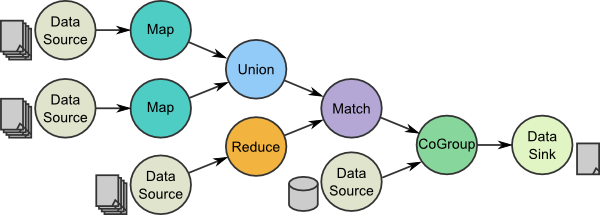
\includegraphics[scale=0.5]{./resources/dataflow}
    \caption{An example of a complex dataflow \cite{pactModel}}
\end{figure}

Directed Acyclic Graphs can also be composed together, by connecting the output of one graph to the input of the next.

The classic MapReduce paradigm could be emulated by having 2 tasks, one with the Map Input Contract and another with the Reduce Input Contract (neither would have Output Contracts). The result of the Map task would be piped directly in to the Reduce task. 

\subsection{Stratosphere}
Stratosphere is the reference implementation of the PACT programming model. It is a runtime environment which takes a Directed Acyclic Graph specifying the desired data processing workflow (the Job Graph) and and compiles it in to an Execution Graph - a more concrete description with information about how the tasks will be made parallel and what types of computing resources will be used \cite{warneke2011exploiting}. 

A secondary focus of the Stratosphere runtime is to take advantage of the opportunities afforded by Cloud Computing. The core benefit of Cloud Computing is elasticity, allowing resources to be obtained on demand. By removing the assumption that resources must be static throughout the duration of a data processing job, Stratosphere is able to utilise the dynamic resource allocation made possible by the cloud. This changes the emphasis of task scheduling, allowing the scheduler to determine and acquire what resources a given task needs, rather than attempting to schedule tasks depending on the resources available at the time \cite{warneke2011exploiting}.

Stratosphere was previously known as Nephele, and research papers from the beginning of the Stratosphere project will refer to it by this name.

%\section{Alternative Technologies}
%There are various alternative data processing technologies which will not be considered in any more detail in this project. 

%\subsection{Google MapReduce}
%Google MapReduce is a proprietary implementation of the MapReduce idea. It originates from the original paper on MapReduce, 

%\subsection{Dryad}

%\section{Summary}